\documentclass[12pt, a4paper]{jarticle}
\setlength{\topmargin}{0cm}
\setlength{\oddsidemargin}{5mm}
\setlength{\evensidemargin}{5mm}
\setlength{\textheight}{23cm}
\setlength{\textwidth}{38zw}
\setlength{\parindent}{1zw}

\usepackage[dvipdfmx]{graphicx,color}
\usepackage{amsthm}
\usepackage{amsmath,amssymb} 
\usepackage{here}
\usepackage{alltt}
\usepackage{enumerate}
\usepackage{url}

\title{各国のモバイル端末のOSのシェアとGDP}
\author{226x105x 大森嶺}
\date{2022年6月12日}
\begin{document}
\maketitle

\section{導入}
現在,日常の様々な部分で多くの人がスマートフォンのアプリや,サービスを利用している.
そのため,アプリケーションや,ソフトを開発する上で,OSのシェアについて把握,理解できていることは重要である.
また,モバイル端末のOSのシェア率について,世界の多くの国ではAndroidの占める割合が高いが,
日本ではiOSの占める割合が高いと言われている.

そこで,日本,他の国についてもOSのシェア,その要因について,
各国のOSのシェア率,人口,一人当たりの GDP を可視化することで,その関係や特徴を調べる.

\section{手法}
各国のOSのシェア率と人口を積み上げ棒グラフ,GDPを折れ線グラフで表示し,
世界地図上でGDPとその国のOSのシェアが最も高いOSがわかるようなカラーマップで表示する.
ここで,世界地図で選択されている国のみを棒グラフ,折れ線グラフに表示するようにする.

また,より詳細に調べられるようにGDPの高い国を$1 \sim 10,11 \sim 20,21 \sim 30$番までを表示し,
その際に人口の上限,下限を設けてフィルタリングできるようにする.

\section{結果}
図\ref{fig:map_os}からほとんどの国で最も利用されているOSがAndroidであることがわかる.
この中でiOSが最もシェアが高い国は,
日本,オーストラリア,アメリカ,カナダ,スイス,スウェーデン,ノルウェイ,デンマークの8カ国のみである.
図\ref{fig:bar_ios}からこの中でGDPが最も低い国は日本である.

GDPの高い順番の21番から30番を見ると,日本が21番になっている.
よって,GDPの上位30カ国のうち,iOSのシェアが最も高い国は8カ国となっている.
ここで,人口に下限を設けてiOSのシェアが最も高い国すべてがGDPの上位10カ国に入る,
もしくは,人口のフィルタによって漏れるようにする.
図\ref{fig:bar_filter}から人口の下限を10,000,000にすると
スイス,ノルウェイ,デンマーク以外の5カ国が上位10カ国に入り,日本が10番目となることがわかる.

また,地図からAndroidのシェアが最も高いような,GDPの高い国とGDPの低い国をランダムに選択する.
図\ref{fig:high_gdp}と図\ref{fig:low_gdp}からiOSのシェアが最も高い国以外で見てみても,GDPの高い国では比較的iOSのシェア率が高くなっていることがわかる.

\begin{figure}[H]
  \centering
  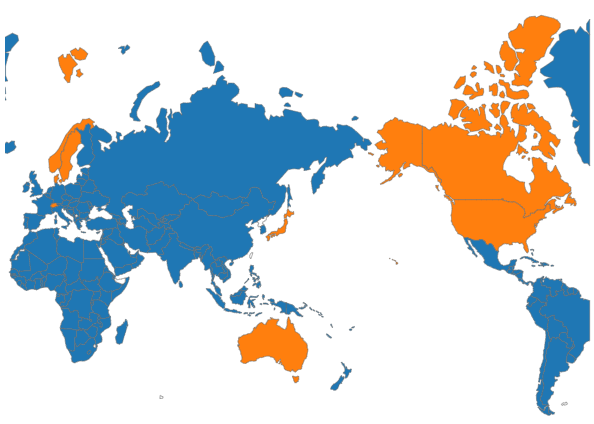
\includegraphics[keepaspectratio, scale=0.8]{imgs/map_os.png}
  \caption{Top OS of each country}
  \label{fig:map_os}
\end{figure}

\begin{figure}[H]
  \centering
  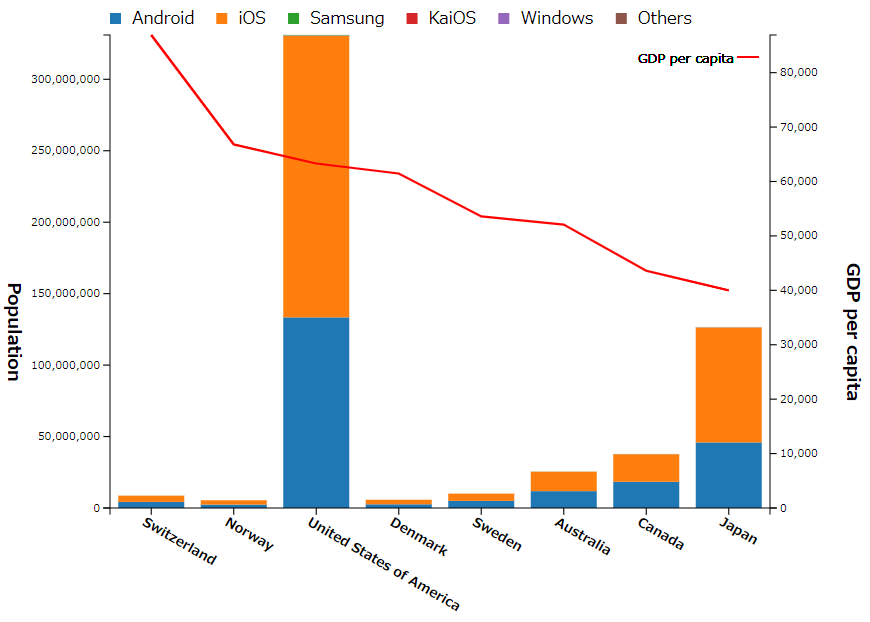
\includegraphics[keepaspectratio, scale=0.6]{imgs/bar_ios.png}
  \caption{GDP of iOS countries}
  \label{fig:bar_ios}
\end{figure}

\begin{figure}[H]
  \centering
  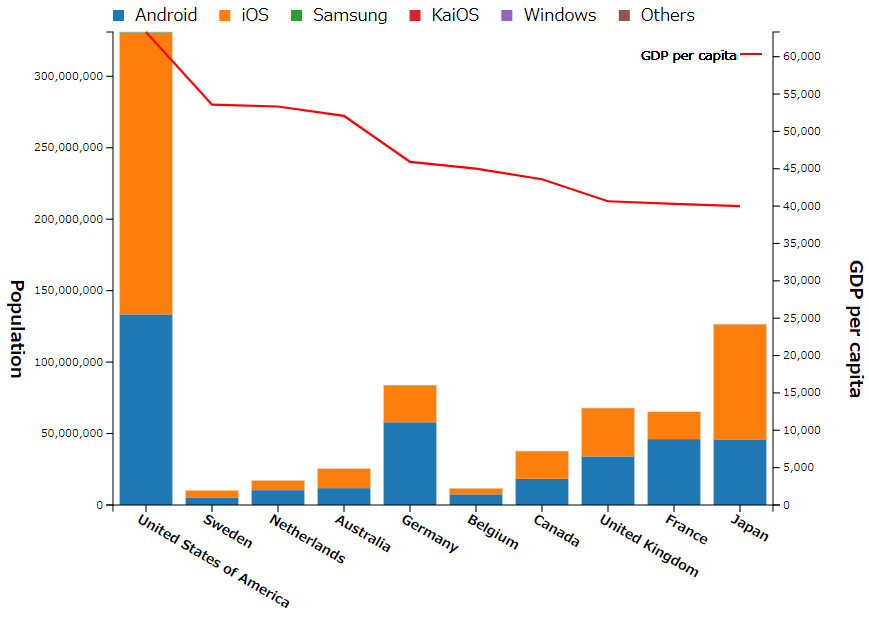
\includegraphics[keepaspectratio, scale=0.6]{imgs/bar_filter.png}
  \caption{High GDP countries filtered by Population}
  \label{fig:bar_filter}
\end{figure}

\begin{figure}[H]
  \centering
  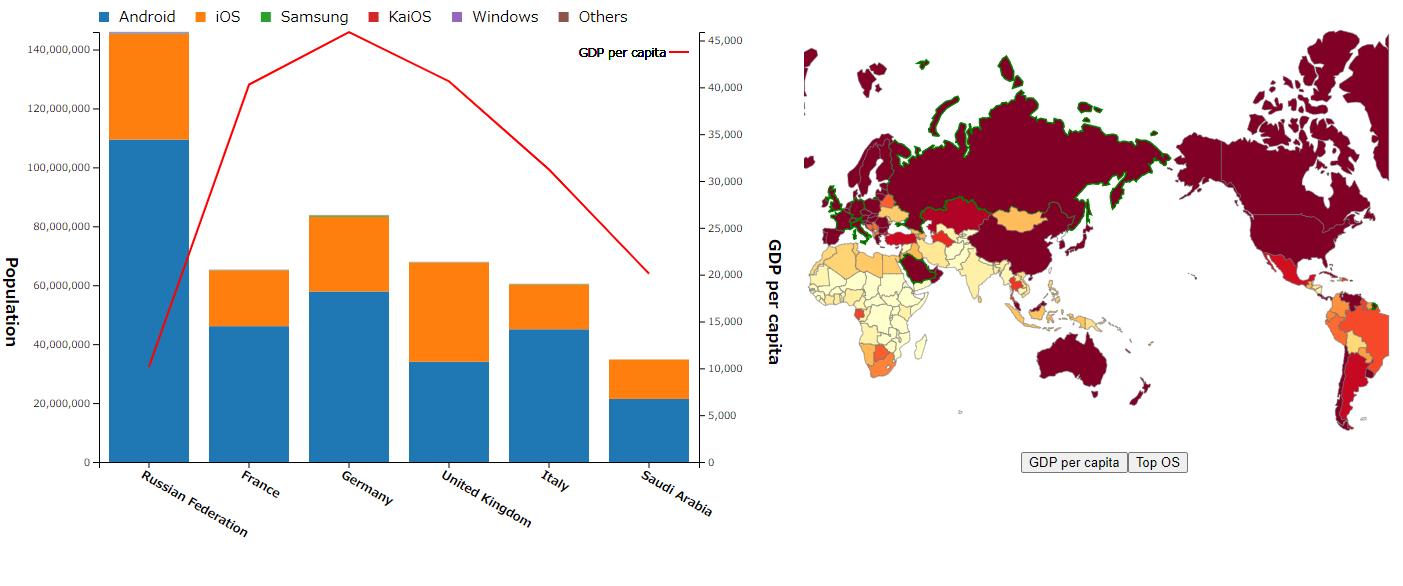
\includegraphics[keepaspectratio, scale=0.33]{imgs/high_gdp.png}
  \caption{High GDP countries}
  \label{fig:high_gdp}
\end{figure}

\begin{figure}[H]
  \centering
  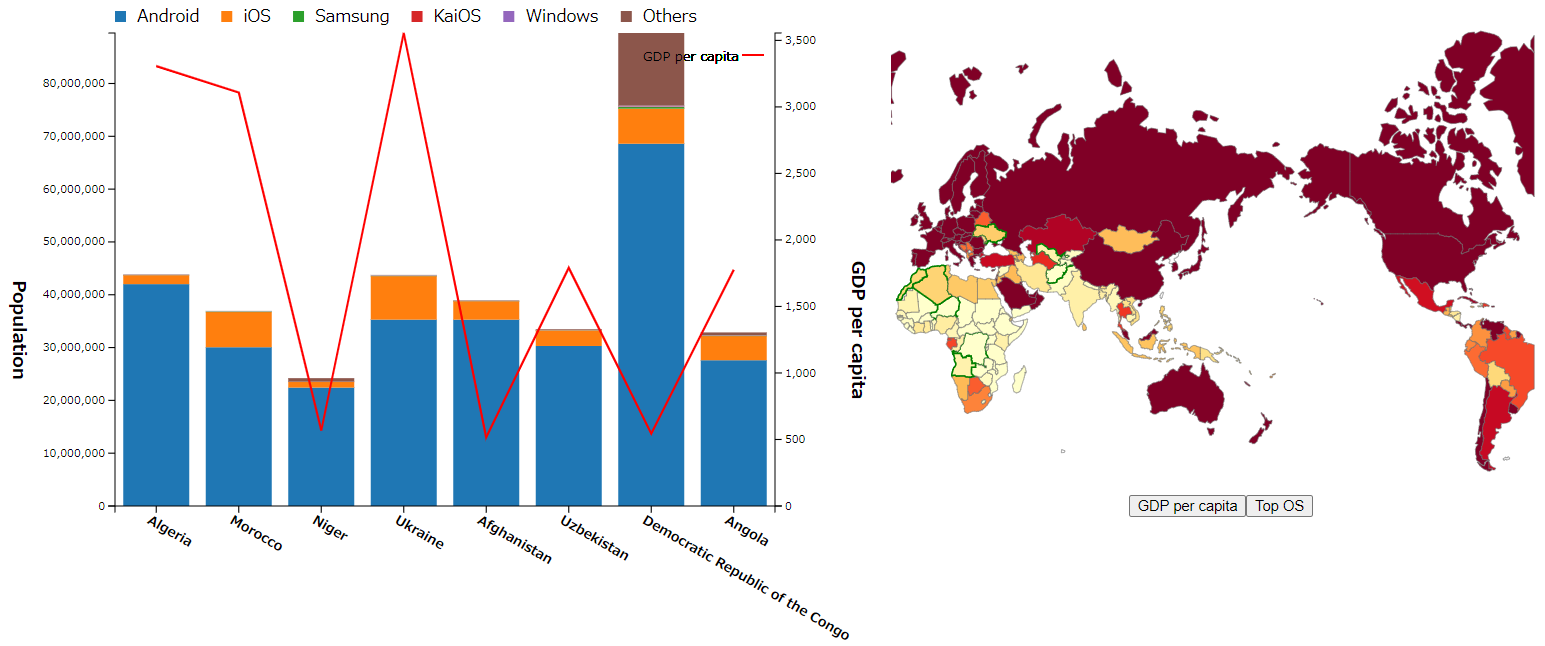
\includegraphics[keepaspectratio, scale=0.3]{imgs/low_gdp.png}
  \caption{Low GDP countries}
  \label{fig:low_gdp}
\end{figure}

% \begin{tabular}{cc}
%   \begin{minipage}[]{0.45\hsize}
%     \begin{center}
%     \end{center}
%   \end{minipage}&
%   \begin{minipage}[]{0.45\hsize}
%     \begin{center}
%     \end{center}
%   \end{minipage}
% \end{tabular}

\section{考察}
GDPの高い順番の21番から30番を見ると,iOSのシェアが最も高い国の中でGDPの最も低い日本が21番目になっている.
iOSのシェアをトップとする8カ国がGDPの上位21カ国に入っていることからGDPが高いことと,
その中でも人口がある程度多い国であることがiOSを利用する割合の高くなる要因であると考えられる.

\section{結論}
人口当たりのGDPの高い国では,低い国に比べてiOSを利用している割合が高くなることが分かった.
よって,これらの国に向けるアプリケーション,サービスではそれを考慮して開発を進めることも必要になる.

\begin{thebibliography}{}
  \bibitem{map_shape} Country boundary

  \url{https://github.com/stamen/spatial-dataviz-for-data-scientists/blob/master/data/world/world-110m.geojson}
  \bibitem{os_data} Mobile Operating System Market Share, statcounter
  
  \url{https://gs.statcounter.com/os-market-share/mobile/worldwide}
  \bibitem{pop_data} World Population, United Nations

  \url{https://population.un.org/wpp/Download/Standard/Population/}
  \bibitem{gdp_data} GDP, The World Bank
  
  \url{https://data.worldbank.org/indicator/NY.GDP.MKTP.CD}
\end{thebibliography}

\end{document}